\section{Desarrollo Experimental 2}
Para realizar este experimento debemos solicitar en el laboratorio el circuito que se muestra a continuación, el cual cumple la condicion de ser un generador de corriente constante manteniendo la corriente a 100 mA. El circuito esta compuesto por los siguientes componentes:
\begin{figure}[H]
    \centering
    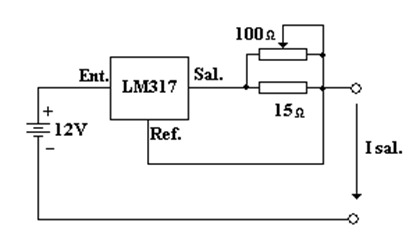
\includegraphics[width=0.4\textwidth]{images/circuitoCA.jpeg}
  \begingroup
\renewcommand{\figurename}{Circuito}
\caption{Experimento 2.}
\label{circuito2}
\endgroup
\end{figure}

\begin{figure}[H]
    \centering
    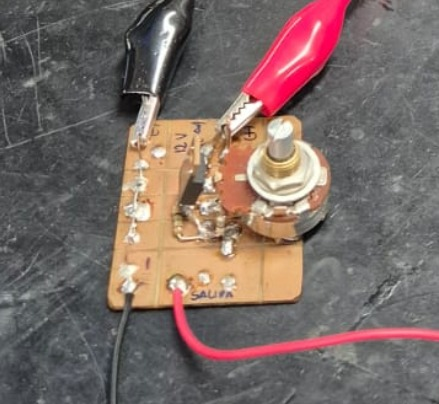
\includegraphics[width=0.4\textwidth]{images/fuentelab.jpeg}
  \caption{Fuente de alimentación del laboratorio}
  \label{fig:fuentelab}
\end{figure}
Para la probeta de ensayo se utiliza un segmento de cable con longitud predeterminada en nuestro caso es de 20m $\pm$ 20cm. Con el fin de facilitar su manipulación, el cable debe enrollarse sin embargo, para evitar efectos inductivos no deseados, se implementa un enrollamiento especial.
Esta probeta es la encargada de ser la resistencia que se desea medir y por la cual van a pasar los 100 mA, esta se conecta al circuito mostrado recientemente.

\begin{figure}[H]
  \centering
  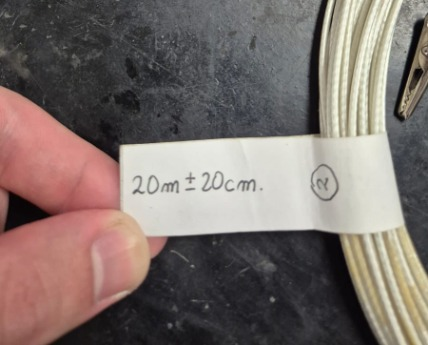
\includegraphics[width=0.4\textwidth]{images/probeta.jpeg}
  \caption{Dimensiones de probeta}
  \label{fig:dimensiones_probeta}
\end{figure}
A continuación, se conecta el circuito a la fuente
ajustada a 12 V, y se calibra mediante el potenciómetro de 100 $\Omega$
hasta obtener una corriente de salida lo más cercana posible a 100 mA.
Para medir la corriente se utiliza el multímetro digital en su función de amperímetro en una escala de 600 mA. En este caso, se logró obtener una corriente de 100,4 mA, lo cual es aceptable para nuestros propósitos experimentales.

\begin{figure}[H]
    \centering
    \includegraphics[width=0.5\textwidth]{images/100mA.jpeg}
  \caption{Corriente de 100,4 mA en una escala de 600 mA.}
  \label{fig:100mA}
\end{figure}

Una vez calibrado el circuito, se procede a medir la tensión en la probeta utilizando un multímetro digital. Con la corriente constante de 100,4 mA, se logra una tensión de 105mv, lo que nos permitirá calcular la resistencia utilizando la ley de Ohm.

$$R = \frac{V}{I} = \frac{105mV}{100,4mA} \approx 1.046 \Omega$$

Ahora para calcular la incertidumbre de la medicion debemos considerar la exactitud de las mediciones de tensión y de corriente de nuestro multímetro ya que La incertidumbre en la determinación de la resistencia por el método propuesto, se vincula con los errores que pueden estar presentes en cada una de las mediciones implicadas en el procedimiento. Para ello utilizamos la hoja de datos de nuestro multímetro digital, el cual tiene una exactitud de $\pm$ (0.5\% + 4 dígitos) para la medición de tensión en la escala de 600 mV y una exactitud de $\pm$ (0.8\% + 8 dígitos) para la medición de corriente en la escala de 600 mA.
\begin{figure}[H]
    \centering
    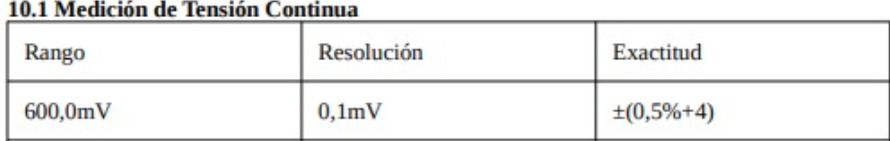
\includegraphics[width=0.5\textwidth]{images/rango600mv.jpeg}
  \caption{Exactitud del multímetro digital.}
  \label{fig:tabla_multimetroram}
\end{figure}

\begin{figure}[H]
    \centering
    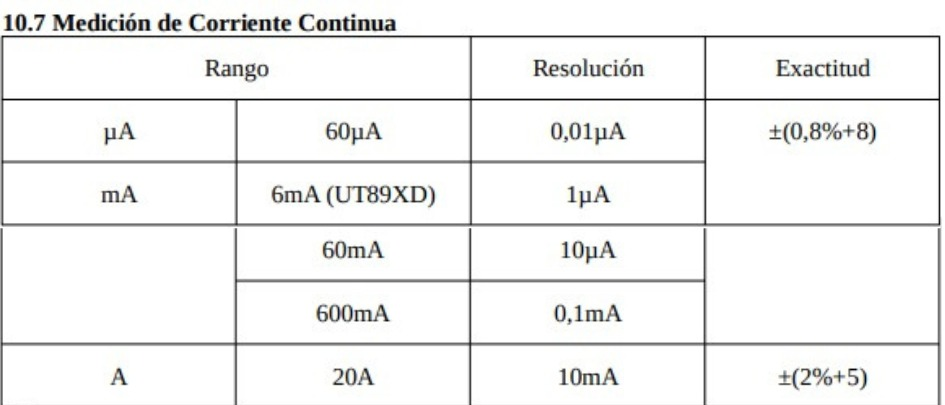
\includegraphics[width=0.5\textwidth]{images/rango600mA.jpeg}
  \caption{Exactitud del multímetro digital.}
  \label{fig:tabla_multimetroram}
\end{figure}

Una vez conocidas las exactitudes, se procede a calcular la incertidumbre de cada medición.
\begin{equation*}
\begin{split}
    \Delta V &= 105mV \cdot \frac{0.5}{100} + 4 \cdot 0.1mV \\
    \Delta V &= \pm0.925mV \\
    \Delta I &= 100.4mA \cdot \frac{0.8}{100} + 8 \cdot 0.1mA \\
    \Delta I &= \pm0.8032mA \\
\end{split}
\end{equation*}
Con esto ya podemos calcular la tabla de valores final.
\begin{table}[h]
\centering
\renewcommand{\arraystretch}{1.8}
\begin{tabular}{|c|c|c|c|c|}
\hline
---- & X & $\Delta x$ & $\frac{\Delta x}{X}$ & $\frac{\Delta x}{X} \cdot 100$ \\ \hline
\textbf{V} & 105 mV & 0.925 mV & 0.0088 & 0.88\% \\ \hline
\textbf{I} & 100.4 mA & 1.6032 mA & 0.0159 & 1.59\% \\ \hline
\textbf{R = V/I} & 1.046 $\Omega$ & 0.0093 $\Omega$ & 0.0089 & 0.89\% \\ \hline
\end{tabular}
\end{table}
